%!TEX root = ../rapport.tex
%!TEX encoding = UTF-8 Unicode

% Chapitres "Introduction"

% modifié par Francis Valois, Université Laval
% 31/01/2011 - version 1.0 - Création du document


\label{s:experimentation}
\chapter{Laboratoire 1}
\section{Projet 1}

L'objectif fondamental de ce laboratoire est de déterminer le potentiel électrique en chaque point d'un système qui présente les caractéristiques montrées sur la figure 1 de l'énoncé de laboratoire. 

\paragraph{} On sait de la physique électrique que l'équation de Laplace pour des éléments infinitésimaux s'écrit comme suit:

\begin{equation}
\label{eq:1}
\nabla ^2 V = 0
\end{equation}

\paragraph{}Or, dans la pratique, il est très difficile d'implanter des méthodes de calculs qui utilisent des équations symboliques. Les géométries réelles présentent certaines difficultés de modélisation et il est beaucoup plus commode de les représenter par des niveaux discrets. Or, il est possible de réécrire les équations obtenues pour une modélisation symbolique selon des équations discrètes. 

\paragraph{}Soit une fonction $V(x,y,z) = f_1(x)f_2(y)f_3(z) $ en coordonnées cartésiennes. L'équation \ref{eq:1} peut se développer comme suit:

\begin{equation}
\frac{\nabla ^2 V}{V} = \frac{1}{f_1}\frac{\partial^2 V}{\partial x^2} + \frac{1}{f_2}\frac{\partial^2 V}{\partial y^2} + \frac{1}{f_3}\frac{\partial^2 V}{\partial z^2}
\end{equation}

\paragraph{} Soit un maillage d'analyse qui correspond à un plan de type (x,y), tel que la figure 1 présentée dans l'énoncé du laboratoire. Si on pose $a$ comme le pas entre deux points d'analyse, on peut effectuer une approximation d'ordre 1 de chacune des dérivées secondes. Pour une dérivée:

\begin{align}
\left[ \frac{\partial^2 V}{\partial x}\right]_{(0,0,0)} &= \frac{1}{a}\left( \left[ \frac{\partial V}{\partial x}\right]_{(a/2,0,0)} - \left[ \frac{\partial V}{\partial x}\right]_{(-a/2,0,0)} \right)
\end{align}

Au moyen d'une approximation d'ordre 1, on obtient:

\begin{align}
\left[ \frac{\partial^2 V}{\partial x}\right]_{(0,0,0)} &= \frac{1}{a}\left( \frac{V_{(a,0,0)} - V_{(0,0,0)}}{a} - \frac{V_{(0,0,0)} - V_{(-a,0,0)}}{a} \right)\\
&\approx \frac{1}{a^2} \left( V_{(-a,0,0)} + V_{(a,0,0)} - 2 V_{(0,0,0)} \right)
\end{align}

On utilise la même logique pour la dérivée seconde dans l'axe y et on négligera celle en z puisque le repère d'analyse ne présente pas de coordonnées en z.
 
\begin{align}
\left[ \frac{\partial^2 V}{\partial x}\right]_{(0,0,0)} &\approx \frac{1}{a^2} \left( V_{(0,-a,0)} + V_{(0,a,0)} - 2 V_{(0,0,0)} \right)
\end{align}

La solution discrète de l'équation de laplace dans le domaine d'analyse concerné est donné par:

\begin{equation}
V_{(0,0,0)} \approx \frac{1}{4} \left(V_{(-a,0,0)} + V_{(a,0,0)} + V_{(0,-a,0)} + V_{(0,a,0)} \right)
\end{equation}

\paragraph{}Les développements précédents sont valides seulement dans le cas où il n'y a qu'un diélectrique (quand on est a l'intérieur d'un diélectrique). Il va de soi que lorsqu'on fait intervenir la notion d'interface entre deux surfaces et de continuité, il faut adapté les équations en conséquences. On obtient l'équation de Laplace que si $\nabla \epsilon = 0$. Dans le cas où plusieurs diélectriques entrent en jeu, cela n'est plus vérifié.  

\paragraph{}Afin de compléter l'analyse des bases théoriques utiles afin de réaliser cette expérience, on effectue l'analyse au moyen du théorème de Gauss du potentiel en un point. La surface d'analyse est un primse rectangulaire de dimensions $a \times a \times \Delta z $, où $\Delta z$ est une hauteur infinitésimale. On suppose qu'il n'y a pas de charges résiduelles en chaque point. Le théorème de Gauss s'exprime alors comme suit:

\begin{equation}
\oint_S D \cdot dS = \oint_S \epsilon E \cdot dS = -\oint_S \epsilon \nabla V \cdot dS  = 0
\end{equation}

Le résultat précédent conduit à un résultat qui est valide pour tous les points du plan d'analyse du laboratoire:

\begin{equation}
V_{(0,0,0)} = \frac{V_{(-a,0,0)} + V_{(a,0,0)}}{4} + \frac{\epsilon_{r1} V_{(0,-a,0)} + \epsilon_{r2} V_{(0,a,0)}}{2(\epsilon{r1} + \epsilon_{r2})}
\end{equation}

Ce qui termine l'analyse du passage des solutions aux équations continues vers les solutions utilisant la théorie des différences finies et appliquées à ce laboratoire.
\section{Projet 2}

La fonction MDF écrite utilise une méthode par relaxation. 

\subsection{Algorithme}
\begin{lstlisting}
function V  = mdf(m, n, er1, er2, d, w, tol)
    
    %Creation des matrices et des variables
    V = zeros(n+1, m+1);
    permitivityMatrix = zeros(n+1, m+1);
    oldMatrix = zeros(n+1, m+1);
    tolerence = false;
    
    %Remplissage des permitivites
    if d == 0; 
        permitivityMatrix(2:n, 2:m) = er2;
    else
        permitivityMatrix(2:n-d, 2:m) = er2;
        permitivityMatrix(n+1-d:n, 2:m) = er1;
    end
    
    %Position du conducteur, de la permitivite du conducteur et du potentiel
    halfW = floor((w+1)/2);
    if mod(m+1,2) == 0
        halfM = (m+1)/2;
    else
        halfM = floor((m+1)/2);
    end    
    V(n+1-d, halfM+1-halfW:halfM+w+1-halfW) = 1;
    
    %Calcul du potentiel de chaque point
    while tolerence == false,
        for i=2:n,
            for j=2:m,
                %Calcul du potentiel du point avec sauvegarde de l'ancienne
                %valeur pour le calcul de tolerence.
                oldMatrix(i,j) = V(i,j);
                
                %Sur le conducteur
                if( i == (n+1-d) && ...
                  ( j >= halfM+1-halfW && j <=  halfM+w+1-halfW))
                    V(i,j) = 1;
                %Sur la ligne de separation du dielectrique
                elseif (i == n+1-d)
                    V(i,j) = (V(i,j-1) + V(i,j+1))/4 + ...
                    (permitivityMatrix(i+1,j) * V(i+1,j) + ...
                    permitivityMatrix(i-1,j) * V(i-1,j))/(2*(er2+er1));
                %Sur le reste
                else
                    V(i,j) = (V(i,j-1) + V(i,j+1) + V(i+1,j) + V(i-1,j))/4;
                end              
            end
        end
        
        %Verification de la tolerence : difference entre chaques matrices
        %et extraction de la valeur maximale
        if(max(abs(oldMatrix - V)) < tol)
            tolerence = true;
        else
            tolerence = false;
        end
    end
    disp(V);
    surf(V);
end


\end{lstlisting}

\subsection{Guide d'utilisation}

\textit{Un fichier nommé mda.m est disponible dans le répertoire remis sur pixel.}
\begin{enumerate}
\item Copier le fichia mda.m dans un répertoire connu du logiciel matlab;
\item Ouvrir le fichier mda.m présent dans le répertoire au moyen de Matlab;
\item Dans l'interpréteur, fixer les paramètres d'appel de la fonction selon la même nomenclature qu'utilisée dans l'énoncé de laboratoire. Pour se faire, utiliser une syntaxe du genre: m=10; etc. 
\begin{itemize}
\item \textit{Exemple:} V = mdf(10,10, 1.10,4,3,$1*10^{(-9)}$);
\end{itemize}
\item Interpréter la ligne (appuyer sur entrer);
\item Une matrice contenant le résultat devrait s'afficher dans l'interpréteur. 
\item Un graphique 3D du potentiel en fonction de la position (x,y) devrait s'afficher.
\end{enumerate}

\subsection{Reproduction des exemples}
\subsubsection{Exemple 7.5}
Pour prouver la validité de notre fonction, il suffit de faire la différence entre chaque point de la matrice de tension obtenue et celle fournie et de vérifier que la différence maximale est en dessous d'un certain seuil. Dans notre cas, nous fixons ce seuil à $10^{-6}$.

La matrice founie est la suivante :

\[V_{prof}  = \left(\begin{array}{ccccccc}
0 & 0 			& 0 			& 0 			& 0 			& 0 			& 0 \\
0 & 0.07043931 	& 0.12599119 	& 0.14570741	& 0.12599119	& 0.07043931 	& 0 \\
0 & 0.15576603 	& 0.28781803 	& 0.33084727 	& 0.28781803 	& 0.15576603 	& 0 \\
0 & 0.26480681 	& 0.53866761 	& 0.60204563  	& 0.53866761 	& 0.26480681 	& 0 \\
0 & 0.36479358 	& 1				& 1				& 1			 	& 0.36479358 	& 0 \\
0 & 0.19436750 	& 0.41267643 	& 0.45633821	& 0.41267643 	& 0.19436750 	& 0 \\
0 & 0 			& 0 			& 0 			& 0 			& 0 			& 0 
\end{array} \right)\]

La matrice obtenu avec un seuil de tolérence de $10^{-9}$ par notre programme est la suivante :
\[V_{MDF}  = \left(\begin{array}{ccccccc}
0 & 0 			& 0 			& 0 			& 0 			& 0 			& 0 \\
0 & 0.07043930 	& 0.12599118 	& 0.14570741	& 0.12599118	& 0.07043930 	& 0 \\
0 & 0.15576603 	& 0.28781803 	& 0.33084727 	& 0.28781803 	& 0.15576603 	& 0 \\
0 & 0.26480681 	& 0.53866761 	& 0.60204562  	& 0.53866761 	& 0.26480681 	& 0 \\
0 & 0.36479358 	& 1				& 1				& 1			 	& 0.36479358 	& 0 \\
0 & 0.19436750 	& 0.41267643 	& 0.45633821	& 0.41267643 	& 0.19436750 	& 0 \\
0 & 0 			& 0 			& 0 			& 0 			& 0 			& 0 
\end{array} \right)\]

Ainsi, en appliquant la différence des deux matrices et en obtenant le résultat maximum, il est possible de vérifer la différence maximale entre ces deux matrices. Dans notre cas, la différence maximale est de $4.5 \cdot 10^{-9}$ ce qui est très en dessous de notre seuil fixé de $10^{-6}$. Cette valeur semble être plus petite que les nombres contenus dans chacune des matrices car pour simplifier la vie du lecteur, nous avons réduits les chiffres significatif présenté dans le rapport mais avons effectué les différents calculs avec les vraies valeurs.

\subsubsection{Exemple 7.6}
La même méthode que l'exemple précédent à été utilisé.

La matrice founie est la suivante :
\[V_{prof}  = \left(\begin{array}{ccccccc}
0 & 0 			& 0 			& 0 			& 0 			& 0 			& 0 \\
0 & 0.06983505 	& 0.12534299 	& 0.14509465	& 0.12534299	& 0.06983505 	& 0 \\
0 & 0.15399721 	& 0.28644227 	& 0.32969262 	& 0.28644227 	& 0.15399721 	& 0 \\
0 & 0.25971150 	& 0.53673627 	& 0.60079129  	& 0.53673627 	& 0.25971150 	& 0 \\
0 & 0.34811255 	& 1				& 1				& 1			 	& 0.34811255 	& 0 \\
0 & 0.18987646 	& 0.41139327 	& 0.45569664	& 0.41139327 	& 0.18987646 	& 0 \\
0 & 0 			& 0 			& 0 			& 0 			& 0 			& 0 \\
\end{array} \right)\]

La matrice obtenu avec un seuil de tolérence de $10^{-9}$ par notre programme est la suivante :
\[V_{prof}  = \left(\begin{array}{ccccccc}
0 & 0 			& 0 			& 0 			& 0 			& 0 			& 0 \\
0 & 0.06983505 	& 0.12534299 	& 0.14509465	& 0.12534299	& 0.06983505 	& 0 \\
0 & 0.15399721 	& 0.28644227 	& 0.32969262 	& 0.28644227 	& 0.15399721 	& 0 \\
0 & 0.25971150 	& 0.53673627 	& 0.60079129  	& 0.53673627 	& 0.25971150 	& 0 \\
0 & 0.34811255 	& 1				& 1				& 1			 	& 0.34811255 	& 0 \\
0 & 0.18987646 	& 0.41139327 	& 0.45569664	& 0.41139327 	& 0.18987646 	& 0 \\
0 & 0 			& 0 			& 0 			& 0 			& 0 			& 0 \\
\end{array} \right)\]

Ainsi, en appliquant la différence des deux matrices et en obtenant le résultat maximum, il est possible de vérifer la différence maximale entre ces deux matrices. Dans notre cas, la différence maximale est de $5.1 \cdot 10^{-9}$ ce qui est très en dessous de notre seuil fixé de $10^{-6}$. Pour la même raison que précédemment, la valeur possède plus de chiffres significatifs que ceux affiché dans le présent rapport dû à l'utilisation de valeurs plus précises que celles présentées.

Ainsi, les deux exemples précédents semblent prouver que la fonction crée possède une précision excellente pour ce qui lui est demandé. Il est donc possible de l'utiliser pour d'autre calculs comme ceux de la section suivante.

\subsection{Programme selon la géométrie et les diélectriques}
Il est important de noter que le programme utilisé n'utilise pas tout à fait la nomenclature mentionné dans l'énoncé du laboratoire. Il est demandé dans l'énoncé que la matrice produite ai son point $(1,1)$ dans le coin inférieur gauche. Toutefois, dans notre cas, la matrice possède son point $(1,1)$ dans le coin supérieur gauche. Ce choix est surtout justifié par la simplification de l'algorithme sachant que les indices de Matlab sont gêrés de cette façon. Ainsi, pour suivre la nomenclature demandé pour les graphiques, l'axe Y à tout simplement été inversé. C'est pourquoi, si l'algorithme est utilisé pour répliquer les graphiques, il va falloir inverser la matrice en Y pour que les axes concordent.

\subsubsection{Diélectrique 1}
Le graphique représenté par la figure \ref{fig1} est le résultat de l'algorithme avec les paramètres suivante : 

\begin{displaymath}
\epsilon_{r1} = \epsilon_{r2} = 1, w= 10 u, d = 4 u
\end{displaymath}
Comme le montre la figure, la vitesse de chute de la tension est en concordance avec $\epsilon$ et w ainsi que d sont bien positionné.

\subsubsection{Diélectrique 2}
Le graphique représenté par la figure \ref{fig2} est le résultat de l'algorithme avec les paramètres suivante : 

\begin{displaymath}
\epsilon_{r1} = \epsilon_{r2} = 1, w= 10 u, d = 20 u
\end{displaymath}
Comme on devait s'y attendre, les pics de tension du conducteur sont déplacé de 16 unités vers le Y positif. De plus, sachant que la seule variable modifiée est la position du conducteur, la courbe possède le même taux de décroissance que la courbe précédente.

\subsubsection{Diélectrique 3}
Le graphique représenté par la figure \ref{fig3} est le résultat de l'algorithme avec les paramètres suivante : 

\begin{displaymath}
\epsilon_{r1} = \epsilon_{r2} = 16, w= 4 u, d = 4 u
\end{displaymath}

Contrairement aux deux courbes précédentes, cette courbe possède un taux de décroissance beaucoup plus élevé dû au $\epsilon$ 16 fois plus grand.

\subsubsection{Diélectrique 4}
Le graphique représenté par la figure \ref{fig4} est le résultat de l'algorithme avec les paramètres suivante : 

\begin{displaymath}
\epsilon_{r1} = \epsilon_{r2} = 16, w= 10 u, d = 4 u
\end{displaymath}

Cette courbe possède le même taux de décroissance que la précédente mais celle-ci possède un conducteur plus long.

\subsubsection{Diélectrique 5}
Le graphique représenté par la figure \ref{fig5} est le résultat de l'algorithme avec les paramètres suivante : 

\begin{displaymath}
\epsilon_{r1} = \epsilon_{r2} = 16, w= 20 u, d = 4 u
\end{displaymath}
Cette courbe possède le même taux de décroissance que les 2 précédentes mais celle-ci possède un conducteur encore plus long soit la moitié du système ce qui rend les tensions aux extrêmité en X plus élevées que les deux courbes précédentes.

\subsubsection{Diélectrique 6}
Le graphique représenté par la figure \ref{fig6} est le résultat de l'algorithme avec les paramètres suivante : 

\begin{displaymath}
\epsilon_{r1} = 2, \epsilon_{r2} = 1, w= 10 u, d = 4 u
\end{displaymath}
Cette courbe est celle attendue pour un système possèdant deux diélectriques distincts. Dans notre cas les deux diélectriques ne diffèrent que d'une permitivité unitaire ce qui ne se voit pas amplement sur le graphique mais qui tout de même fait varier la décroissance plus ou moins vite en fonction de la position en X et Y.

\subsubsection{Diélectrique 7}
Le graphique représenté par la figure \ref{fig7} est le résultat de l'algorithme avec les paramètres suivante : 

\begin{displaymath}
\epsilon_{r1} = 16, \epsilon_{r2} = 1, w= 10 u, d = 4 u
\end{displaymath}

Cette dernière courbe est sensiblement pareille que la précédente mais cette fois ci, la différence de permitivité entre les deux diélectriques est de 16.
\begin{figure}
	\centering
	\mbox{
		\subfigure[Diélectrique 1]{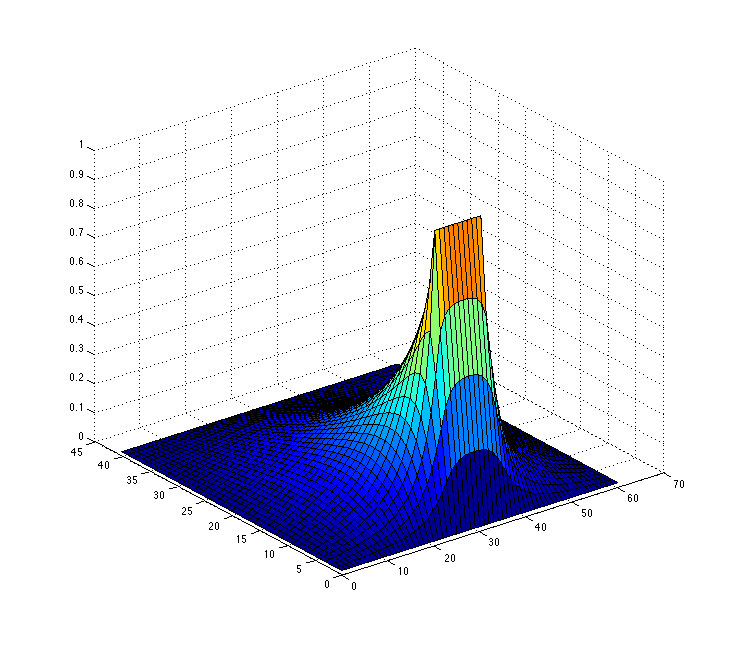
\includegraphics[width=3in]{graph1.png} \label{fig1}}
		\quad
		\subfigure[Diélectrique 2]{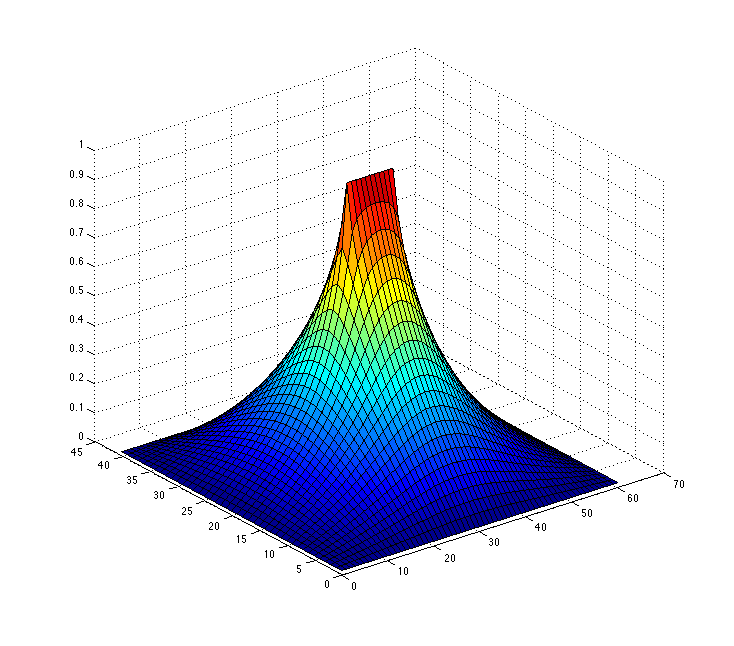
\includegraphics[width=3in]{graph2.png} \label{fig2}}
	}
\end{figure}
\begin{figure}
	\centering
	\mbox{
		\subfigure[Diélectrique 3]{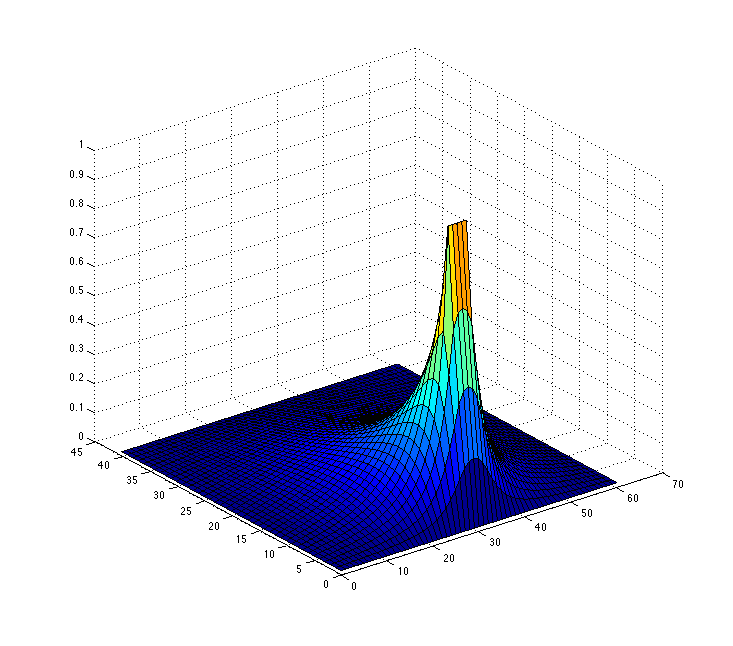
\includegraphics[width=3in]{graph3.png} \label{fig3}}
		\quad
		\subfigure[Diélectrique 4]{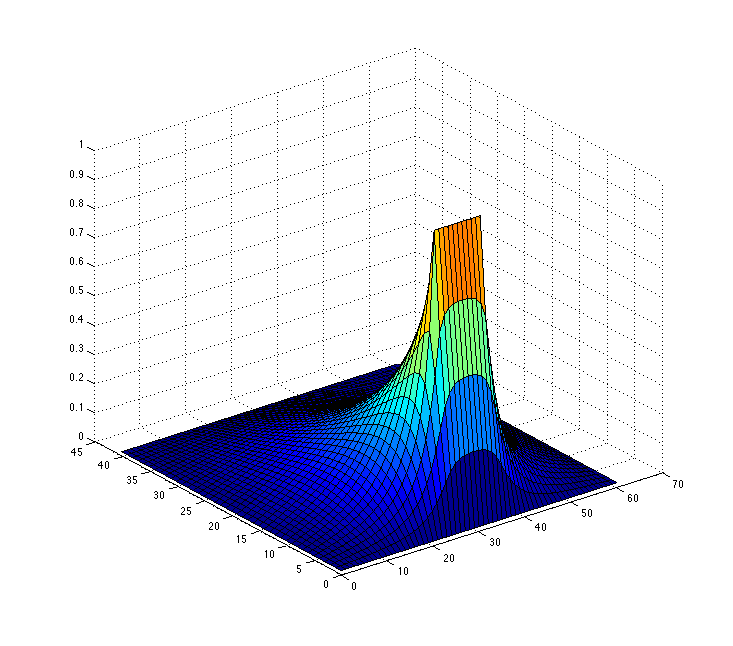
\includegraphics[width=3in]{graph4.png} \label{fig4}}
	}
\end{figure}
\begin{figure}
	\centering
	\mbox{
		\subfigure[Diélectrique 5]{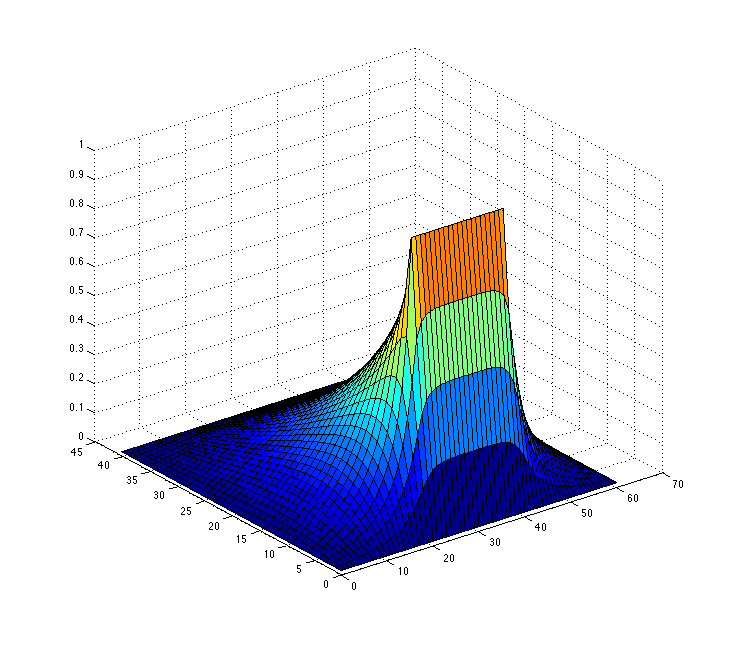
\includegraphics[width=3in]{graph5.png} \label{fig5}}
		\quad
		\subfigure[Diélectrique 6]{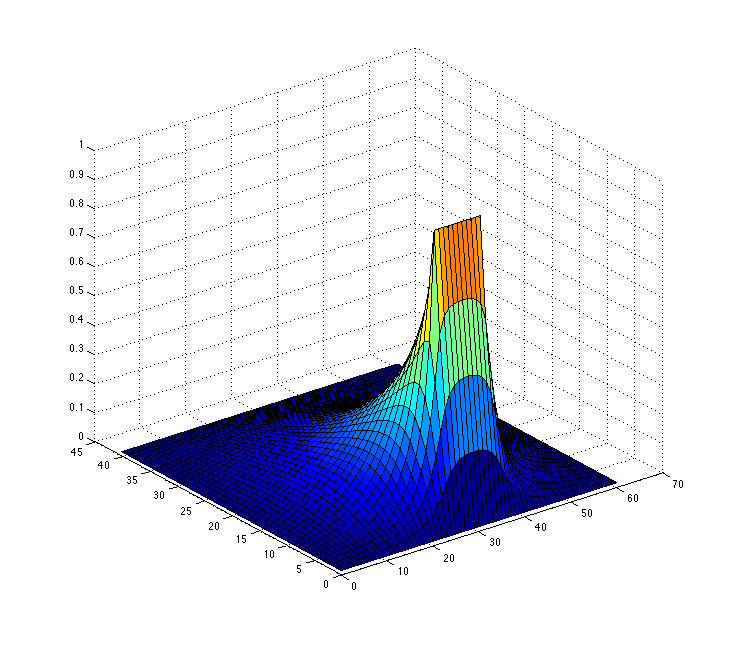
\includegraphics[width=3in]{graph6.png} \label{fig6}}
	}
\end{figure}
\begin{figure}
	\centering
	\mbox{
		\subfigure[Diélectrique 7]{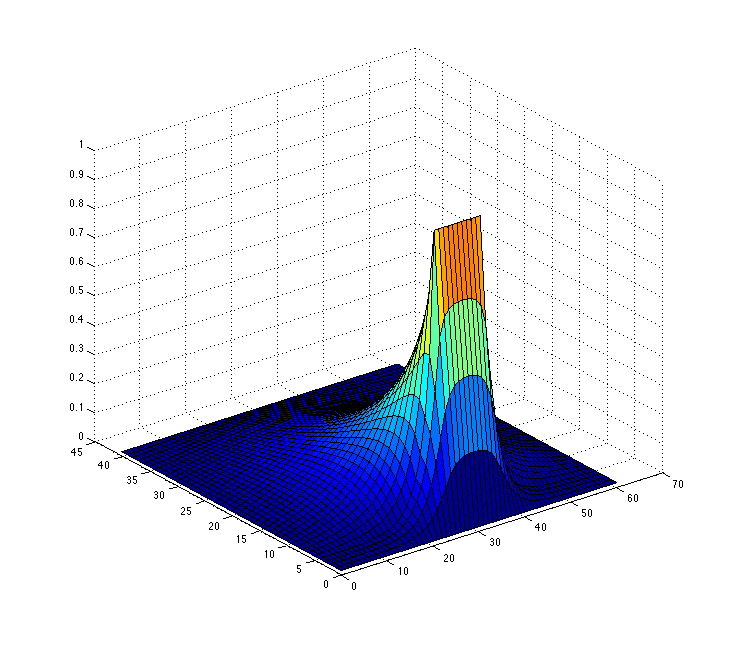
\includegraphics[width=3in]{graph7.png} \label{fig7}}
	}
\end{figure}